\documentclass[11pt]{article}
\usepackage{graphicx}
\usepackage{caption}
\usepackage{subfig}
\usepackage{geometry}
\usepackage{amsfonts}
\usepackage{amsmath}
\usepackage{amsthm}
\usepackage{xcolor}

\newcommand{\abs}[1]{\lvert #1 \rvert}
\usepackage{indentfirst}
\newtheorem{lemma}{Lemma}[section]
\geometry{letterpaper, portrait, margin=1in}
\setlength{\parindent}{0cm}
\numberwithin{equation}{section}
\numberwithin{figure}{section}
\begin{document}

\setlength\parindent{24pt}

\begin{center}


625.721 Final Project: Simulation of Wind Direction over the Atlantic Ocean

\null

Matthew LeDuc


\end{center}
\section{Introduction}

The theory of statistics on convex subsets of $\mathbb{R}^n$ has been studied since at least the 7th century, when the Arab scholar Al-Khalil used permutations and combinations to list all possible Arabic words with and without vowels \cite{Broemling}. However, there are several areas relevant to daily life when the methods of linear statistics break down completely. For example, we know that the time halfway between 23:00 and 01:00 hours is 00:00 hours, however taking the average of 23 and 1 leads us to believe that the halfway time is 12:00 hours. We also know that the compass direction between 315 degrees (NW) and 45 degrees (NE) is not 180 degrees (S) but actually 0 deg (N), a difference of 180 degrees! Setting your compass this way would leave you hopelessly lost (ask me how I know). For this reason, over the last century the field of directional or circular statistics has been growing incredibly rapidly, starting with Richard von Mises studying the deviation of atomic weights from integer values and continuing into the present day \cite{Mardia2}.  At present, the field finds applications in modeling of temporal variations in environmental phenomena such as wind and wave direction, in the modeling of the migration patterns of birds, protein folding, and in any other area that can be assumed to be taking place on $\mathbb{S}^n$, the $n-$cylinder, or the $n-$torus. Many great examples of these sorts of processes can be found in the references, in particular in \cite{Craig}, \cite{Kanti}, and \cite{Mardia2}. 

Many papers have focused on the modeling of distributions of wind direction (see \cite{Al Yammahi}, \cite{Craig}, and \cite{Mahrt}, among many others, for examples). This is of particular interest to many people in industry and government, who want to know how such variations might affect, for example, the output of a wind power plant. We will continue to follow this trend in this paper. We will investigate the use of these techniques on data from the National Data Buoy Center to model time series of wind direction measured over the ocean.

\section{Circular Statistics}

\section{Distributions on the Circle}

Now that we have seen the basics of circular statistics, we will introduce the most important circular probability distributions. 

\subsection{The circular uniform distribution}

The easiest generalization from the real line to the circle is the uniform distribution. This is given by the probability density

\begin{equation}\label{uniformpdf}
f_X(x) = \frac{1}{2\pi} 
\end{equation}
which has the associated distribution function 

\begin{equation}\label{uniformcdf}
F_X(x) = \frac{x}{2\pi}
\end{equation}

This has all the same properties as the uniform distribution of the real line, so we will not spend time discussing it in detail. 

\subsection{The von Mises Distribution}
There are several different distributions that can be used for modeling wind direction data, however the most common is the von Mises distribution \cite{Al Yammahi}. Its probability density function is given by

\begin{equation}\label{eq:vm}
f_{X}(x) = \frac{e^{\kappa \cos(x - \mu)}}{2\pi I_0(\kappa)}
\end{equation}
and its cumulative density function is given by \cite{Kanti}

\begin{equation}\label{eq:vmcdf}
F_X(x) = \frac{1}{I_0(\kappa)}\int_0^x e^{\kappa \cos(x-\mu)}dx
\end{equation}

where $\mu$ is the angular mean, $\kappa \in [0,\infty)$ is a parameter that determines the spread of the distribtuion, and $I_0(\kappa)$ is the zeroth order modified Bessel function of the first kind given by 

\begin{equation}\label{eq:I0}
I_r(\kappa) = \frac{1}{2\pi} \int_0^{2\pi}\cos( r \theta )e^{\kappa\cos(\theta )} d\theta, r = 0,\pm 1, \pm 2,...
\end{equation}

We will denote the von Mises distribution with parameters $\mu$ and $\kappa$ by $M(\mu, \kappa)$.

\subsubsection{Maximum Likelihood Estimation}

We will determine the approximate distribution of the wind direction via maximum likelihood estimation. Consider a set of $n$ data points $ x_1, x_1, ...,x_n $that are drawn from some distribution $f_X(x;\theta)$ where $\theta$ is an unknown parameter or vector of parameters. We can estimate $\theta$ by means of maximizing the likelihood function of the distribution. The likelihood function for $\theta$ is given by

\begin{equation}\label{eq:likelihood fn}
L(\theta) = \prod_{k=1}^n f_X(x_k|\theta)
\end{equation}

and the maximum likelihood estimate is the value $\hat{\theta}$ such that $L(\hat{\theta}) \ge L(\theta)$ for all values of $\theta$ and is the solution of the equation $\nabla L(\theta) = 0$, or equivalently $\nabla \log(L(\theta)) = 0$ (called the log-likelihood) which can often reduce the difficulty of the computation \cite{Larsen}. The log-likelihood function for the von Mises distribution given $n$ data points is given by 

\begin{equation}\label{eq:vmll}
\log(L(\kappa, \mu)) = -n\log( 2\pi I_0(\kappa))+ \sum_{k=1}^n e^{\kappa \cos(x_k-\mu)}
\end{equation}

Taking the appropriate gradient and setting it to zero, we can derive the maximum likelihood estimators $\hat{\mu}$ and $\hat{\kappa}$. Let the data points $x_1, x_2, ..., x_n$ be drawn from the interval $[0,2\pi)$ according to some distribution and consider the transformation $z_k = e^{i x_k}$. Then the smaple mean is given by $\bar{z} =\frac{1}{n}\sum_{k=1}^n z_k$ and the maximum likelihood estimate for $\mu$ is given by $\hat{\mu} = \textnormal{Arg}(\bar{z})$. The estimator for $\kappa$ is given by \cite{borradaile}

\begin{equation}
\label{eq:kmle}
\bar{R} = \frac{I_1(\hat{\kappa})}{I_0(\hat{\kappa})}
\end{equation}

where $\bar{R} = \|\bar{z}\|$. This equation can be solved via your favorite rootfinding algorithm. For the purposes of this paper, the Newton-Rhapson method was used.  

In order to model a time series of von Mises random variables, we will also need to understand the distribution of the difference of two von Mises variables. First, we will determine the distribution of a negative von-Mises random variable. 

\begin{lemma}\label{nvm}
If $X\in M(\mu, \kappa)$ then $W = -X \in M(-\mu,\kappa)$.
\end{lemma}

The proof is as follows: Let $X\in M(\mu, \kappa)$ be a random variable and let $W = -X$. Then $F_W(w) = P(W\le w) = P(-X\le w) = 1-P(X\le -w) = 1-F_X(-w)$, where $F_X(x)$ is as given in equation \ref{eq:vmcdf}. By definition, the probability density of $W$ is given by

\begin{equation}\label{eq:wpdf}
f_W(w) = \frac{d}{dw}\left( 1-\frac{1}{2\pi I_0(\kappa)}\int_0^{-w}e^{\kappa \cos(x-\mu)}dx \right)
\end{equation}

This derivative can be readily evaluated to show that $f_W(w) = \frac{1}{2\pi I_0(\kappa)}e^{\kappa \cos(w+\mu)}$ which is the PDF for a $M(-\mu, \kappa)$ random variable.

With the aid of Lemma \ref{nvm}, we can determine the distribution of the difference between two von Mises random variables. Let $X \in M(\mu, \kappa)$ and $Y \in M(-\mu, \kappa)$. Since $-Y \overset{d}{=}X$ the distribution of the sum $X+Y$ is identical to the distribution of $X-X_1$ where $X_1 \overset{d}{=}X$. Letting $Z = X+Y$, we can apply the convolution theorem for sums of random variables and follow the derivation contained in \cite{Kanti} of teh distribution of the sum of two von Mises random variables. 

\begin{equation}\label{eq:rvsum}
f_Z(z) = \int_0^{2\pi}f_X(x)f_Y(z-x)dx
\end{equation}

From this, we can see that 

\begin{equation}\label{eq:vmsum}
f_Z(z) = \frac{1}{(2\pi I_0(\kappa))^2}\int_0^{2\pi} e^{\kappa(\cos(x-\mu)+\cos(z-x+\mu))}
\end{equation}

We can apply trigonometric identities to show that $\kappa (\cos( x-\mu )+\cos( z-x+\mu )) = \kappa (\cos(\mu)+\cos(z+\mu))\cos( x ) +\kappa(\sin(\mu)+\sin( z+\mu )\sin(x)$. Then we can show that the distribution $f_Z(z)$ is given by 

\begin{equation}\label{eq:sumdist}
f_Z(z) = \frac{1}{2\pi I_0(\kappa)^2}I_0\left ( \sqrt{ 2\kappa^2(1+\cos(z)) } \right)
\end{equation}

This is not a von Mises distribution, however we can still make use of it in the coming sections.

\section{Time Series Analysis of Circular Data}

One straightforward way to determine the time correlation of the data is by using the formulation of the correlogram given in \cite{fisher}. They define the sample correlogram $\rho$ as

\subsection{Periodograms of circular data}

Since we will want to detect periodic behavior in the time series, we will use the formulation for the periodogram of circular data given in \cite{Craig}, which is an estimate of the spectrum of a zero-mean stochastic process with length $n$. The periodogram of the zero mean process $\{x_k\}$ is given by 

\begin{equation}\label{eq:pgram}
\hat{g}(p) = \frac{1}{n}\left |{ \sum_{k=1}^n x_j \exp(i 2 \pi p k/n ) }\right | ^2
\end{equation}
 We can detect periodicity by the relative size of $\hat{g}$. When $\hat{g}(p)$ is large there is more energy contained in the component of the process with normalized frequency $p/n$, and when it is small there is less energy. If ${x_k}$ is sampled with sampling frequency $f_s$, the real frequencies are given by $f = \frac{p}{n}f_s$. 

Since any sequence of angles can be considered as a sequence of points along the unit circle, we can easily extend this formulation to circular data. Given a sequence of angles $\{x_k\} \in \left [0,2\pi \right)$ the stochastic process $\{z_k = \exp(i x_k)\}$ lies on the unit circle, and we can readily calculate its mean $\mu$ using equation CITE EQUATION. Armed with this knowledge, it is readily seen that the periodogram of circular data is given by 

\begin{equation}\label{eq:cpgram}
\hat{g}(p) = \frac{1}{n}\left |{ \sum_{k=1}^n (z_j-\mu) \exp(i 2 \pi p k/n ) }\right | ^2
\end{equation}

\subsection{ARMA processes on the circle}

\begin{equation}\label{eq:fishcor}
\rho(k) = 
\end{equation}

\section{Modeling}

Over rthe years, a variety of models have been introduced for generating data with a proper directional distribution. 

\subsection{Markov Processes on the Circle }

In \cite{Johnson} , Johnson and Wehrle developed an algorithm for generating stationary Markov processes on the circle. Consider three distributions on the circle given by $f_1(\theta),f_2(\phi), g(\cdot)$ and let $F_k(\theta)$ be the distribution function of $f_k$. The distribution $g(\cdot)$ is called the binding density. We wish to find a joint distribution function $f(\theta, \phi)$ such that the marginal densities are $f_1$ and $f_2$. Johnson and Wehrle showed that 

\begin{equation}\label{eq:xtion}
 f_{\Theta, \Phi}(\theta, \phi) = 2\pi g\{ F_{\Theta}(\theta)  -  F_\Phi(\phi) \}f_\Theta(\theta)f_\Phi(\phi)
\end{equation}
satisfies this condition. This can be seen by substituting $z = F_k( x )$ and integrating to calculate the marginals. They went on to define a Markov process on the unit circle by choosing $f=f_1=f_2$ and setting the initial density $p(\theta_0) = f(\theta_0)$. We can clearly see from equation \ref{eq:xtion} that the conditional density of each $\theta_t$ is 

\begin{equation} \label{eq:xdensity}
p(\theta_t | \theta_{t-1}, \theta_{t-2}, ..., \theta_0) = p(\theta_t | \theta_{t-1} )=  2\pi g\{ F(\theta_t)  -  F(\theta_{t-1}) \}f(\theta_t)
\end{equation}
since each $\theta_t$ has the same marginal distribution.

We can use this to apply the Metropolis-Hastings algorithm \cite{Metropolis} to generate data that is distributed as $f$. Let $\{\Theta_t\}$ be a sequence of random variables on the set $I = [0,2\pi)$ with target distribution $f(\theta)$. First, choose some value $y \in I$ from the transitional density $p(y|\theta_t)$ given in equation \ref{eq:xdensity}. Now, let

\begin{equation}\label{eq:alpha}
\alpha = \min\{1,\frac{f(y)p(y|\theta_t)}{f(\theta_t)p(\theta_t|y)}\}
\end{equation}

\begin{figure}[h]
\centering
\subfloat[Uniform binding, $\kappa = \frac{1}{2}$]{
  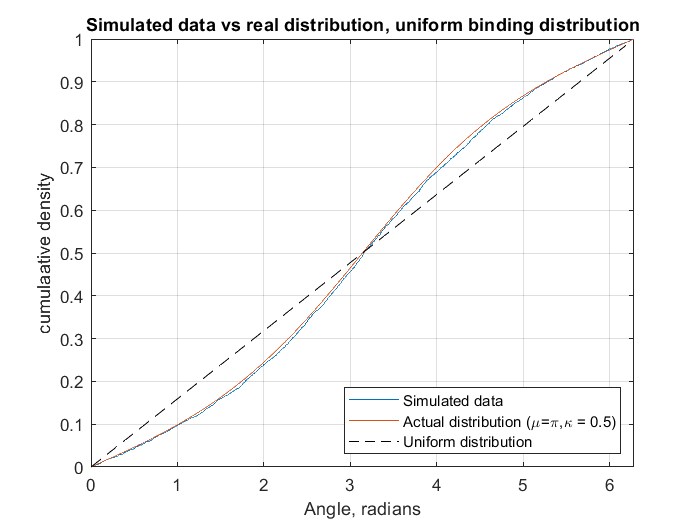
\includegraphics[width=65mm]{New Folder/MH vs real uniform binding.png}
}
\subfloat[Von Mises binding, $\kappa = \frac{1}{2}$]{
  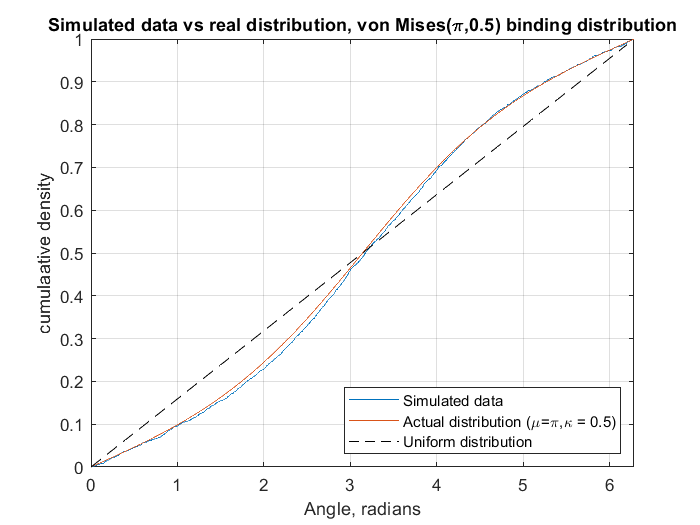
\includegraphics[width=65mm]{New Folder/MH vs real vm binding.png}
}
\newline
\subfloat[Uniform binding, $\kappa = 2$]{
  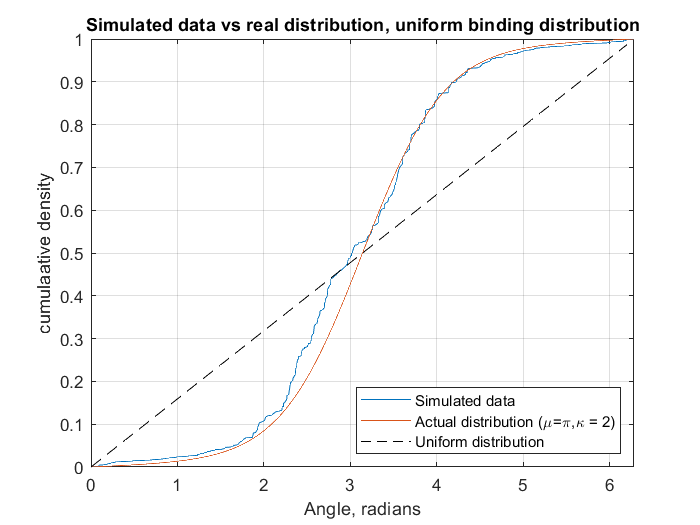
\includegraphics[width=65mm]{New Folder/MH vs real uniform 2 binding.png}
}
\subfloat[Von Mises binding, $\kappa = 2$]{
  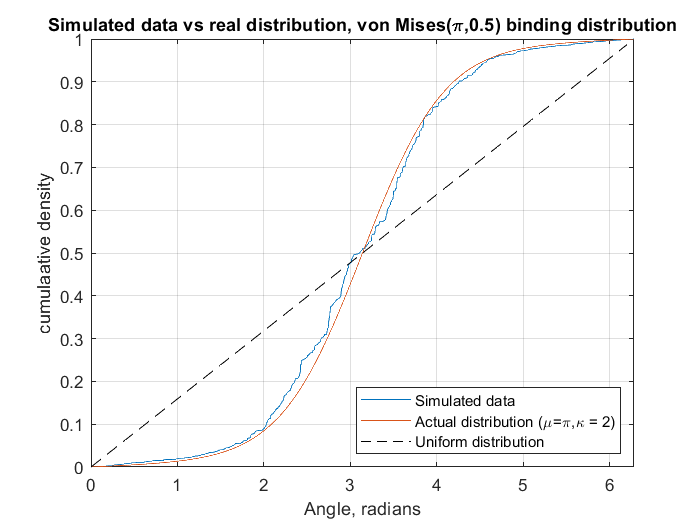
\includegraphics[width=65mm]{New Folder/MH vs real vm 2 binding.png}
}
\caption{Simulated data vs target distribution for various distributions and binding densities, $n=4000$}\label{fig:mhexamples}
\end{figure}

Then, set $\theta_{t+1}=y$ with probability $\alpha$ and $\theta_{t+1}=\theta_t$ with probability $1-\alpha$, and step forward. The expression in $\alpha$ can be thought of as a sort of likelihood function, where values of $y$ that are more "likely" to have come from $f(\theta)$ than $\theta_t$ get accepted automatically and others only get accepted with some probability $\alpha <1$ depending on their similarity to the expected distribution. Results for $\theta \in M(\mu = \pi, \kappa = \{\frac{1}{2}, 2\})$ with $n=4000$ and both a uniform and $M(\pi,\frac{1}{2})$ binding density are shown in figure \ref{fig:mhexamples}. Based purely on these results it appears that for larger values of $\kappa$ the distribution of $\{\Theta_t\}$ converges to the target distribution more slowly. 

This is a nice result, however in order to simulate realistic data our model must also have realistic autocorrelation. As we can see in figure \ref{fig:mh ac}, the simulated data has almost no autocorrelation, but data from NDBC buoys is highly autocorrelated. We will discuss ways to remedy this in the next section by introducing circular autoregressive models. 

\begin{figure}
\centering
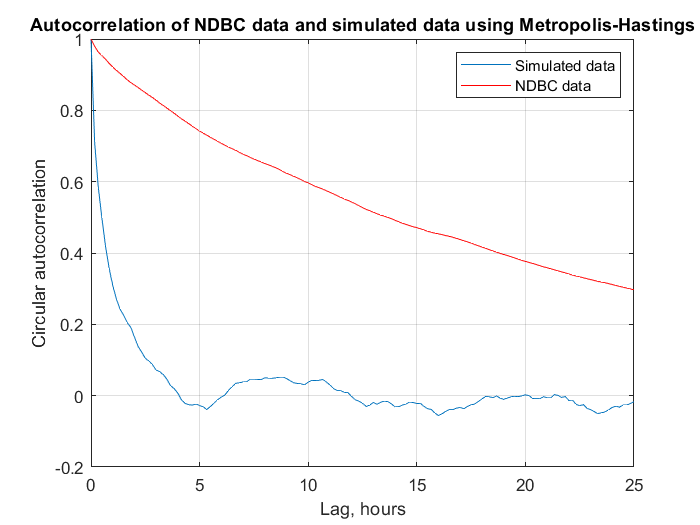
\includegraphics[width=85mm]{New Folder/ac data v model.png}
\caption{Autocorrelation of data generating using Metropolis-Hastings vs real data}\label{fig:mh ac}
\end{figure}

\subsection{Circular Autoregressive Models}

\textcolor{red}{remove?}

\subsubsection{Wrapped and Linked Processes}
There are several ways to generate autocorrelated circular data in the literature. One of the more common approaches is the wrapped autoregressive (WAR(p)) processs, by which a Gaussian process $\{x_t\}$ on the real line is converted to a circular time series by setting

\begin{equation}\label{eq:WAR}
y_t = x_t (\textnormal{mod } 2\pi)
\end{equation}

These models can be seen as a missing data problem: The unwrapped observations can be written as $x_t = y_t+2\pi k_t$ where $k_t$ is an integer \cite{Harvey}. Estimation can be done via expectation maximization, which can be very difficult for any somewhat complex model. There are Markov Chain Monte Carlo methods to do this fitting proposed in \cite{Coles}. 

A second commonly employed model is the linked or circular ARMA(p,q) process (LARMA(p,q)  or CARMA(p,q) ) \cite{Harvey}. This method associates a linear time series model $x$ to a circular time series $y$ with mean $\mu$ by means of a link function $g(t)$ via

\begin{equation}\label{eq:larma}
x = g^{-1}(y-\mu)
\end{equation}
where $g(t)$ is an increasing function on $\mathbb{R}$ with range $2\pi$ such that $g(0)-g(-\infty) = \pi$. The most common link functions are probit transformations given by $g(x) = (2 \Phi( x )-1)\pi+\mu$, where $\Phi(x)$ is the normal CDF, or functions of the form $g(x) = 2\arctan(x)+\mu$. If the aim is to have $x$ be nearly Gaussian, the probit transformation is preferred. In these models the inverse of $x$ is caled an inverse autoregressive process (IAR(p)) in which the conditional mean of a circular distribution is given by \cite{Harvey}

\begin{equation}\label{IAR}
\mu_{t|t-1} = \mu+g\{\phi_1g^{-1}(y_{t-1}-\mu)+...+\phi_p g^{-1}(y_{t-p}-\mu)\}
\end{equation}

When $p=1$ and $\phi_1 \approx 1$ we can rewrite the IAR(1) model as

\begin{equation}\label{eq:IAR1}
\mu_{t|t-1} \approx \mu+\phi_1(y_{t-1}-\mu)
\end{equation}

This shows us that when $\phi_1 = 1$, $\mu_{t|t-1} = y_{t-1}$ so our process is a random walk \cite{Harvey}. However, there is one significant issue with this approach: it ignores that $y=0$ is the same point as $y=2\pi$, and it makes it impossible to jump directly from, for example, $y=\epsilon$ to $y=2\pi-\delta$ in spite of the fact that those values are actually close to each other. The next section describes one attempt to resolve this problem.

\subsection{Score-driven Models}

The next class of models is based on the use of a score function to dynamically update an equation for the conditional mean at each time step. This section draws heavily from \cite{Harvey}, which is a thorough discussion of score-driven models. The score function is defined as the gradient of the log-likelihood function, and so for the $M(\mu, \kappa)$ distribution it is given by taking the gradient of equation \ref{eq:vmll}:

\begin{equation}\label{eq:vmscore}
s(\mu,\kappa) = \nabla \log{L_M(\mu, \kappa) } = \begin{bmatrix} \frac{\partial \log L}{\partial \mu} \\ \frac{\partial \log L}{\partial \kappa}  \end{bmatrix}
=\begin{bmatrix} \kappa \sin(x-\mu ) \\ \cos(x-\mu)-R \end{bmatrix}
\end{equation}
where $R$ is the mean resultant length. 

The score function is used as follows. Let $u_t$ be the score of an observation taken at time t and let $\phi<1$ be a parameter. A score-driven update for the conditional mean $\mu_{t|t-1} $ is given by the recurrence relation
\begin{equation}\label{eq:score update}
\mu_{t|t-1} = (1-\phi)\mu+\phi \mu_{t-1|t-2}+a u_{t-1}
\end{equation}
where $a$ is a parameter that determines the influence of the score on the updating and $\mu$ is the unconditional mean of the random variable. When $a=0$ this expression has a fixed point at $\mu_t = \mu$. The effect of the score function is such that if the score of step $t-1$ is large, the next step will be large and if it is small, the next step will be smaller. 

This can be used to define the conditional distribution of the variable $x_t$ on the real line given by $x_t = \mu_{t|t-1}+\epsilon_t$, where $\epsilon_t$ has zero mean. In the event that an observation falls outside of the support, it can be wrapped to the variable $y_t$ so that it falls in the support. if we have $\epsilon_t \in M(0,\kappa)$, the score $u_t$ is given by

\begin{equation}\label{eq:score mu}
u_t = \sin(y_t-\mu_{t|t-1})
\end{equation}

If, instead of using the conditional mean, we use the unconditional mean $\mu$, we can derive the score-driven circular autoregressive model (SCAR) with order $p$ as

\begin{equation}\label{eq:scar}
\mu_{t|t-1} = \mu+\phi_1 \sin(y_{t-1}-\mu)+...+\phi_p \sin(y_{t-p}-\mu)
\end{equation}

\subsection{Stochastic Differential Equation Models}

Our last (and most successful) potential model candidate comes from the field of stochastic differential equations. A basic stochastic differential equation is the Ornstein-Uhlenbeck process given by

\begin{equation}\label{eq:ornuhl}
d X_t = b(t, X_t)dt+\sigma(t,X_t)dW_t
\end{equation}
where $dW_t$ is a Wiener process, that is, a continuous time stochastic process with independent, normally distributed increments with mean $0$ and variance equal to the time step so that $W_{t+\Delta t}-W_t \in N(0,\Delta t)$. This process is a modification of the continuous random walk, and can be thought of as a continuous analogue to the AR(1) process \cite{oksendal}.

One of the first continuous time processes on the circle was proposed in \cite{Kent1}. This process, known as the von Mises process, can be thought of as a continuous time analogue to the Ornstein-Uhlenbeck process \cite{Garcia}. It was defined as the solution to the familiar looking stochastic differential equation

\begin{equation}\label{eq:vmp}
d \Theta_t = \alpha \sin(\mu - \Theta_t)dt+\sigma dW_t
\end{equation}
where again $W_t$ is a Wiener process, $\alpha>0$ is a drift coefficient, $\mu$ is the mean direction, and $\sigma$ is a diffusion coefficient. This process has a unique stationary distribution given by the $M(\mu, \frac{2\alpha}{\sigma^2})$ distribution. By assuming unit time steps, this can be easily reformulated into a stochastic difference equation as

\begin{equation}\label{eq:sdiff}
\theta_{t+1} - \theta_t = \alpha \sin( \mu - \theta_t )+\sigma \epsilon_t
\end{equation}
where $\epsilon \in N(0,1)$. If we know our stationary distribution, we can develop a model using equation \ref{eq:sdiff} to generate autocorrelated data with the desired distribution. This formulation also allows us to leverage regression techniques to determine the value of $\alpha$. 

An example of the data generated by this model is shown in figure \ref{fig:sdfig}. The data shown consists of 50000 samples generated with a target stationary distribution given by the $M(\pi/4, 2)$ distribution and with $\alpha = 0.01$. The data is strongly autocorrelated with a $1/e$ decorrelation time of approximately 15 hours assuming a sample rate of 6 samples per hour (which aligns with the NDBC data). 

\begin{figure}[h]
\centering
\subfloat[Sample autocorrelation of data generated from a von Mises process]{
  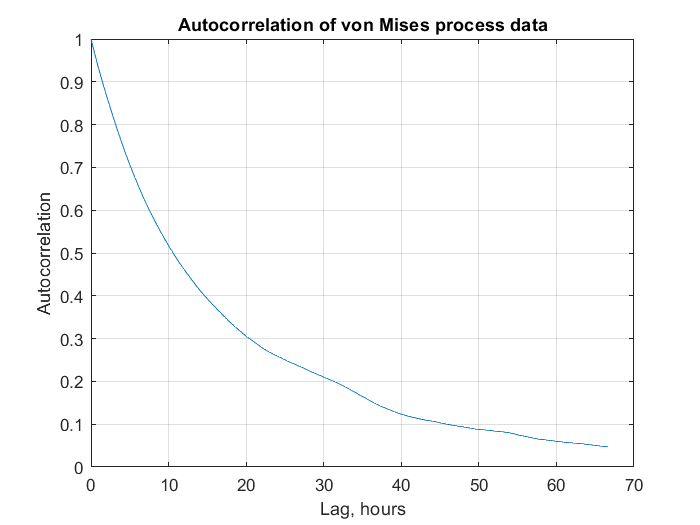
\includegraphics[width=65mm]{New Folder/ac from vm process.png}
}
\subfloat[Simulated data vs stationary distribution]{
  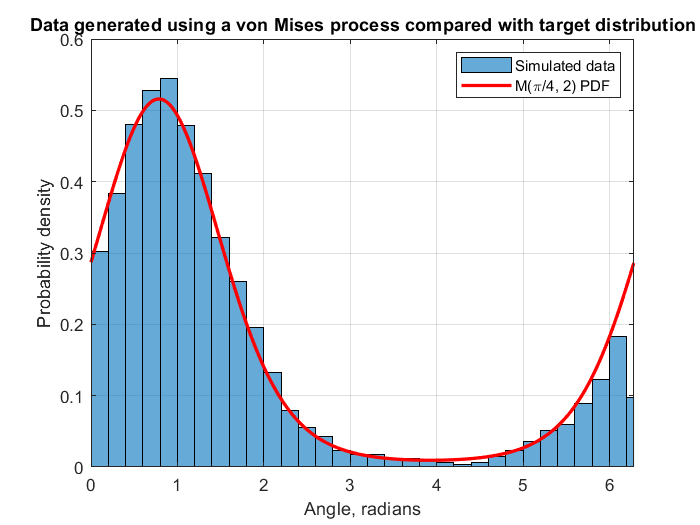
\includegraphics[width=65mm]{New Folder/vm process pdfs.png}}
\caption{Autocorrelation of simulated data and comparison with stationary distribution}\label{fig:sdfig}
\end{figure}

\section{Results}
\section{Conclusions}
\begin{thebibliography}{1}

\bibitem{Al Yammahi} Al Yammahi, Aishah \& Prashanth R. Marpu \& Taha B. M. J. Ouarda (2021), ''Modeling directional distributions of wind data in the United
Arab Emirates at different elevations'', Arabian Journal of Geosciences

\bibitem{Rinaldo} Artes, Rinaldo \& Clelia M. C. Toloi (2009) An Autoregressive Model for Time
Series of Circular Data, Communications in Statistics - Theory and Methods, 39:1, 186-194, DOI:
10.1080/03610920802650338

\bibitem{borradaile} Borradaile, G. J. (2003). Statistics of earth science data : their distribution in time, space, and orientation. Springer. ISBN 978-3-662-05223-5

\bibitem{Broemling} Broemeling, Lyle D. (1 November 2011). "An Account of Early Statistical Inference in Arab Cryptology". The American Statistician. 65 (4): 255–257. doi:10.1198/tas.2011.10191

\bibitem{Coles} Coles, S. G. (1998). Inference for circular distributions and processes. Statistical Computing, 5

\bibitem{Craig} Craig, Peter S (1988), ''Time Series Analysis for Directional Data'', Phd Thesis

\bibitem{fisher} Fisher, N.I and A.J. Lee (1994), ''Time Series Analysis of Circular Data'', Journal of the Royal Statistical Society. Series B

\bibitem{Garcia}  García-Portugués, Eduardo, Michael Sørensen, Kanti V. Mardia, and Thomas Hamelryck (2019), "Langevin diffusions on the torus: estimation and applications", Statistics and Computing

\bibitem{Harvey} Harvey, Andrew; Hurn,Stan, and Stephen Thiele (2019) "Modeling Directional (Circular) Time Series", https://doi.org/10.17863/CAM.43915

\bibitem{Holzmann} Holzmann H, Munk A, Suster M, Zucchini W (2006) Hidden Markov models for circular and linear–circular
time series. Environ Ecol Stat 13:325–347

\bibitem{Johnson} Johnson RA, Wehrly TE (1979) Bivariate models for dependence of angular observations and a
related Markov process. Biometrika 66:255–2566

\bibitem{Kato} Kato,Shogo (2010); "A Markov Process for Circular Data" , Journal of the Royal Statistical Society. Series B (Statistical Methodology)

\bibitem{Kent1} Kent, J. (1975). Discussion of paper by K. V. Mardia. J. Roy. Statist. Soc. Ser. B, 37(3):377–378

\bibitem{Kuiper} Kuiper, N. H. (1960) "Tests concerning random points on a circle". Proceedings of the Koninklijke Nederlandse Akademie van Wetenschappen, Series A. 63: 38–47.

\bibitem{Larsen}Larsen, Richard J and Morris L. Marx, ''An Introduction to Mathematical Statistics and Its Applications, 6th Edition'', Pearson Education, 2018

\bibitem{Mahrt} Mahrt, Larry (2011) ''Surface Wind Direction Variability'',  Journal of Applied Meteorology and Climatology, 

\bibitem{Kanti}Mardia, Kantil; Jupp, Peter E. (1999). Directional Statistics. Wiley. ISBN 978-0-471-95333-3.

\bibitem{Mardia2} Mardia, K. V. (1975), "Statistics of Directional Data", Read before the Royal Statistical Society at a meeting organized by the Research Section on Wednesday, March 19th, 1975

\bibitem{Metropolis}Metropolis, N., A.  Rosenbluth, M.  Rosenbluth, A.  Teller, and E. Teller (1953), Equation of state calculation by fast computing machines, J. Chem. Phys., 21, 1087-1092

\bibitem{oksendal} Øksendal, Bernt (YEAR), Stochastic Differential Equations: An Introduction with Applications, Springer-Verlag Heidelberg New York



\end{thebibliography}



\end{document}